\documentclass[tikz,border=8pt]{standalone}
\usetikzlibrary{arrows.meta,positioning}
\begin{document}
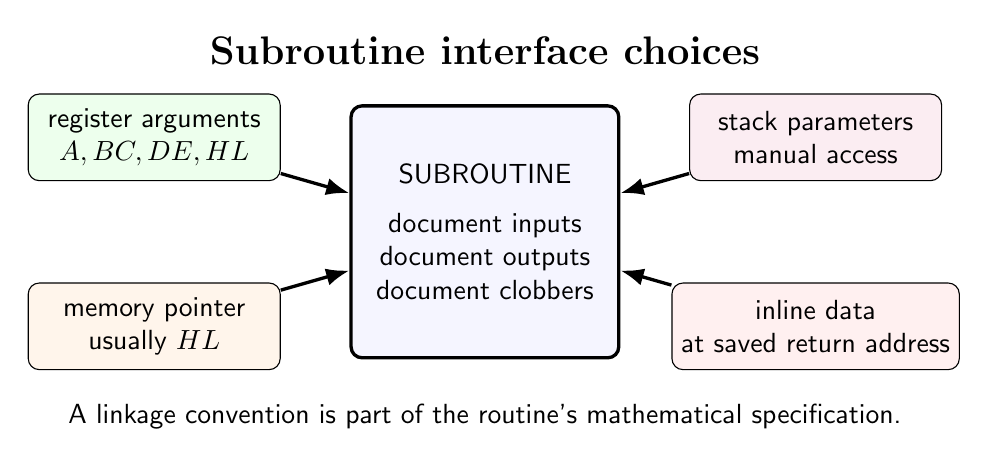
\begin{tikzpicture}[font=\sffamily,>=Latex,source/.style={draw,rounded corners,minimum width=3.2cm,minimum height=1.1cm,align=center},routine/.style={draw,very thick,rounded corners,minimum width=3.4cm,minimum height=3.2cm,align=center,fill=blue!4}]
\node[font=\Large\bfseries] at (6.0,5.0) {Subroutine interface choices};
\node[routine] (r) at (6.0,2.7) {SUBROUTINE\\[2mm]document inputs\\document outputs\\document clobbers};
\node[source,fill=green!7] (reg) at (1.8,3.9) {register arguments\\$A,BC,DE,HL$};
\node[source,fill=orange!8] (ptr) at (1.8,1.5) {memory pointer\\usually $HL$};
\node[source,fill=purple!7] (stk) at (10.2,3.9) {stack parameters\\manual access};
\node[source,fill=red!6] (inline) at (10.2,1.5) {inline data\\at saved return address};
\draw[very thick,->] (reg)--(r);
\draw[very thick,->] (ptr)--(r);
\draw[very thick,->] (stk)--(r);
\draw[very thick,->] (inline)--(r);
\node at (6.0,.35) {A linkage convention is part of the routine's mathematical specification.};
\end{tikzpicture}
\end{document}
